The design patterns likely to be most relevant to \nep \ are described
in refs~\cite{y2re332,y2re333}.

The PUPPETEER pattern appears to be
exclusive to the works of Rouson~et~al, hence is described further here.
It is directed towards the calculation of the Jacobian of multi-component
systems typically needed for Newton-Raphson type solution of update equations.
The idea is that the puppeteer need only know which blocks of the Jacobian
matrix are nonzero, although the puppets need to be capable of forming derivatives
with respect to all state variables.
\begin{figure}
\centerline{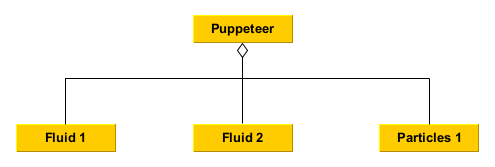
\includegraphics[width=0.95\textwidth]{./pics/puppeteer_wab.png}}
\caption{
PUPPETEER pattern. Each puppet (`Fluid~1', `Fluid~2', `Particles~1') may include terms  involving 
the other puppets. For example, suppose the puppet for `Fluid~1' has terms involving also `Particles~1'
variables (but not `Fluid~2'), then the puppeteer can request derivatives of the puppet's terms both
with respect to `Fluid~1' and `Particles~1' variables, but knows not to ask for derivatives with respect
to `Fluid~2' variables.
\label{fig:puppeteer_wab}}
\end{figure}
